\documentclass{article}
% ready for submission
\usepackage{neurips_2023}
\usepackage{biblatex} %Imports biblatex package
\addbibresource{sample.bib} %Import the bibliography file


% to compile a preprint version, e.g., for submission to arXiv, add add the
% [preprint] option:
%     \usepackage[preprint]{neurips_2023}


% to compile a camera-ready version, add the [final] option, e.g.:
%     \usepackage[final]{neurips_2023}


% to avoid loading the natbib package, add option nonatbib:
%    \usepackage[nonatbib]{neurips_2023}


\usepackage[utf8]{inputenc} % allow utf-8 input
\usepackage[T1]{fontenc}    % use 8-bit T1 fonts
\usepackage{hyperref}       % hyperlinks
\usepackage{url}            % simple URL typesetting
\usepackage{booktabs}       % professional-quality tables
\usepackage{amsfonts}       % blackboard math symbols
\usepackage{nicefrac}       % compact symbols for 1/2, etc.
\usepackage{microtype}      % microtypography
\usepackage{xcolor}         % colors


\title{Image Recovery From Underexposed Photographs Using Generative Models}


% The \author macro works with any number of authors. There are two commands
% used to separate the names and addresses of multiple authors: \And and \AND.
%
% Using \And between authors leaves it to LaTeX to determine where to break the
% lines. Using \AND forces a line break at that point. So, if LaTeX puts 3 of 4
% authors names on the first line, and the last on the second line, try using
% \AND instead of \And before the third author name.


\author{
  David S.~Hippocampus
  Department of Electrical & Computer Engineering\\
  University of Califonia San Diego\\
  La Jolla, CA 92093 \\
  \texttt{hippo@cs.cranberry-lemon.edu} \\
  % examples of more authors
  \And
  Sepehr Aiden Bostan\\
  Affiliation\\
  La Jolla, CA 92093\\
  \texttt{sbostanb@ucsd.edu}\\
  \And
  Yiteng Zhao \\
  Affiliation \\
  La Jolla, CA 92093 \\
  \texttt{email} \\
}


\begin{document}


\maketitle

\begin{abstract}
  Low light imagery has been a persistent challenge in fields like photography, computer vision, and feature detection. To address this problem, probabilistic methods and deep generative models such as GANs have emerged as promising solutions. In this paper, we present our approach to recovering underexposed images using GAN-based techniques, while also addressing the shortcomings of existing methods. Our proposed approach improves the quality of recovered images, making them more visually appealing and useful in various applications such as object detection in low light using cameras or simply photography in extremely dark conditions.
\end{abstract}



\section{Introduction}
\subsection{What research problem are we trying to solve?}
The application of Computer Vision and users of social media have driven the demand of clear, vibrant, and well-exposed images under all situations. However, the current CMOS sensors used in cameras and smartphones only performs well under good lighting condition due to physical constrains such as the size of pixels in CMOS sensor and its capability of capturing photons in challenging lighting condition. Insufficient photons received by the CMOS pixels causes low Signal-to-Noise ratio and results in dark images. These dark, under-exposed images are difficult for computer vision analysis and human to perceive contents from them. There are several physical approaches to increase the Signal-to-Noise ratio such as manufacturing bigger pixels, enlarging aperture, increasing ISO, etc.. However, bigger pixels reduces the overall resolution of the image, and enlarging aperture reduces depth of fields, while increasing ISO will introduces awful lots of noise to the image. Our research problem is finding a better method of recovering underexposed images with computation approach using probabilistic neural network model while keeping the image sharp, color-accurate and clean. 

\subsection{Why is this problem important?}
The potential of solving this problem can extend from mere convenience to saving lives. For example, in computer vision and autonomous vehicles, instead of using lidars in low light conditions we can simply use cameras for object detection and obstacle avoidance, similarly for search and rescue operations a similar method can be used, in radiation imagery such as x-ray images used in the medical field loses some amount of details due to underexposed pixels, this can be potentially life-threatening as it could hide a small tumor or other irregularities which would otherwise be detected by medical professionals. On the other hand in photography, underexposed images can be recreated with higher brightness which can merely be convenient for people.
\section{Related Works}

The literature has thoroughly examined the computational processing of low-light images. We will give a brief overview of the methods currently available.

\subsubsection{Convolutional Neural Networks} 
Extreme low light imaging using convolutional neural networks is a novel topic. Researchers have explored the use of deep neural networks \cite{LearningToSeeInTheDark} for image enhancement. The use of deep neural networks for image enhancement has some limitations and shortcomings, as highlighted by several factors. Firstly, the convolutional network is individually tuned for each camera sensor. The model requires cross-sensor generalization to be effective across different cameras. Secondly, the hyper-parameters of the network, in particular the amplification factors, need to be manually tuned, indicating the need for an auto ISO feature to improve efficiency. Thirdly, the absence of HDR tone mapping and dynamic objects in the dataset limits the network's ability to enhance such images. Moreover, there are artifacts present in the final image, which could potentially be reduced. Finally, the long processing time of 0.38-0.66 seconds per image could pose a challenge in real-time applications. Therefore, while deep neural networks offer promising results for image enhancement, these limitations need to be addressed to improve their practicality and effectiveness in various applications.

\subsubsection{Low-light image enhancement.}

There are different techniques for image enhancement, including histogram equalization and gamma correction. Histogram equalization involves balancing the histogram of the entire image, while gamma correction increases the brightness of dark regions and compresses bright pixels. More advanced techniques involve global analysis and processing, such as the inverse dark channel prior, wavelet transform \cite{AutomaticContrastEnhancement}, Retinex model\cite{retinex}, and illumination map estimation. However, these techniques typically assume that the images already have a good representation of the scene content.

However, we are focusing on extreme low-light imaging, which is characterized by high levels of noise and color distortion that exceed the capabilities of current enhancement pipelines.

\section{Methodology}
\subsection{Proposed a solution for solving this problem}
\section{Novelty and significance of our solution}
\section{Tentative timeline}
\begin{figure}[h]
  \centering
  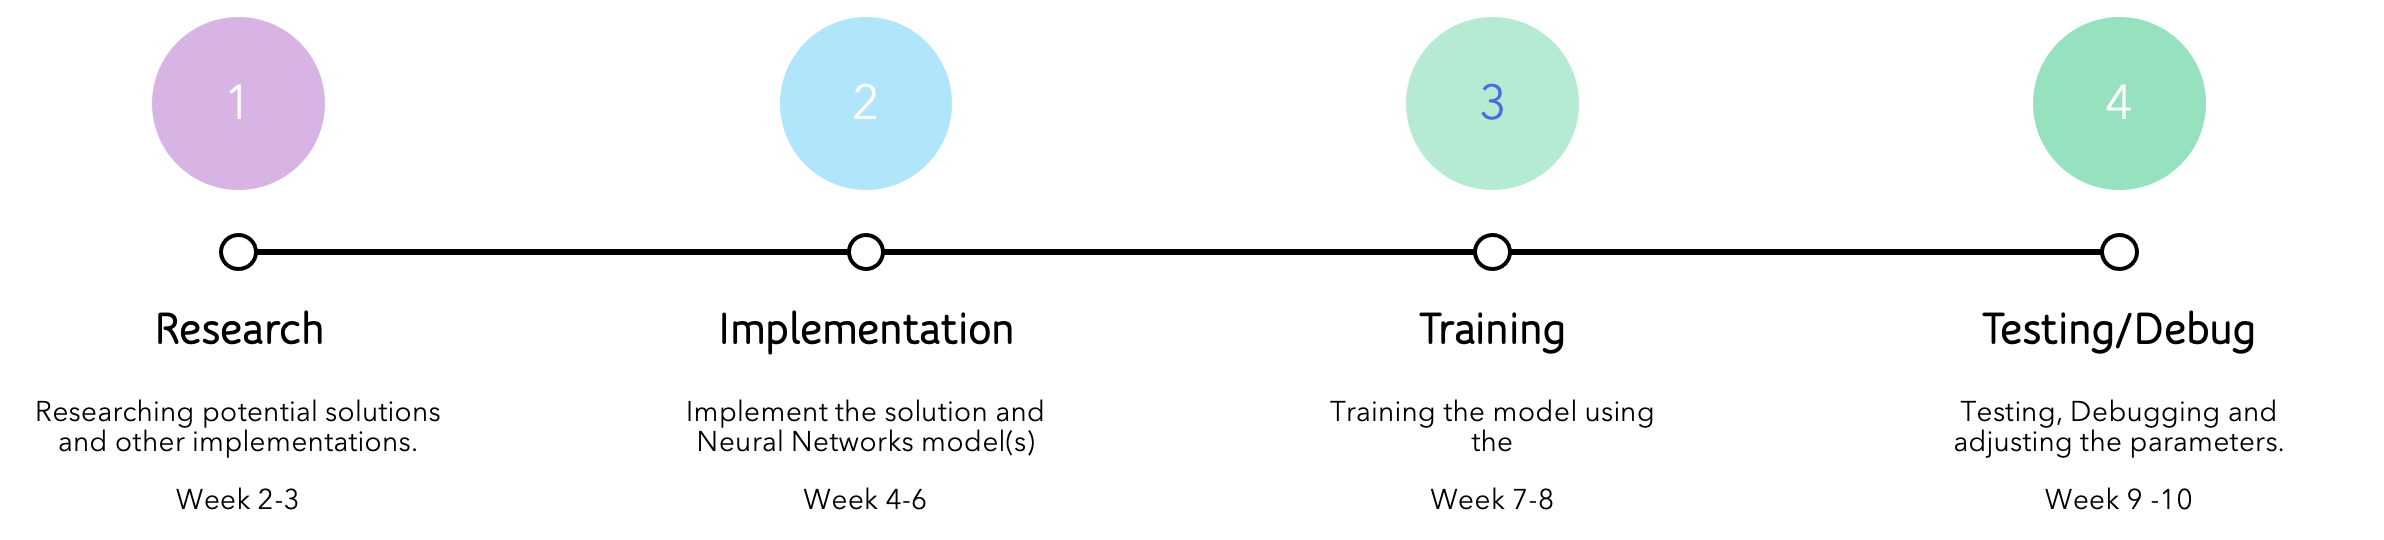
\includegraphics{timeline.png}
  \fbox{\rule[-.5cm]{0cm}{4cm} \rule[-.5cm]{4cm}{0cm}}
\end{figure}
\printbibliography %Prints bibliography
\end{document}